%!TEX TS-program = xelatex
%!TEX encoding = UTF-8 Unicode

% 一定要用 xelatex 進行編譯,字體目前是使用Mac內建的中文字體
% Empty codeblocks will cause formatting problem

%%%%%%%%%%%%%%%%頁面設定%%%%%%%%%%%%%%%%%%%

 %\documentclass[10pt,twocolumn,oneside]{article} %垂直兩欄、單面列印
%\setlength{\columnsep}{14pt} %兩欄模式的間距
%\setlength{\columnseprule}{0pt} %兩欄模式間格線粗細

\documentclass[10pt,oneside]{article}
\usepackage{pdflscape}
\usepackage{multicol}
\usepackage{tocloft}
\renewcommand\cftsecafterpnum{\vspace{-0.6ex}}
\renewcommand\cftsubsecafterpnum{\vspace{-0.6ex}}

\usepackage{pdfpages}

\linespread{1} % 行距

\usepackage{enumitem} % Disable spacing in enumeration list
\setlist{nolistsep}

\usepackage{geometry} %定義邊界
\geometry{a4paper, total={170mm,257mm}, left=10mm, top=20mm, right=10mm}

%%%%%%%%%%%%%%%%%%%%%%%%%%%%%%%%%%%%%%%

\usepackage{pdfpages} %導入pdf文檔, \includepdf[pages={3,4}]{problem_statement.pdf}

\usepackage[colorlinks=true, urlcolor=cyan]{hyperref} %使用超連結, \href{http://codeforces.com/blog/entry/17974}{Codeforces}

\usepackage{fancyhdr}	%設定頁首頁尾

\usepackage{verbatim}  % 大量註解用 , \begin{comment}  % 註解開始,  \end{comment}  % 註解結尾

%%%%%%%%%%%%%%%%中文設定%%%%%%%%%%%%%%%%%%%

\usepackage{fontspec} %加這個就可以設定字體 
\usepackage{xeCJK} %讓中英文字體分開設置
%\setmainfont{Arial}
\setCJKmainfont{STKaiti} %設定中文為系統上的字型,而英文不去更動,使用原TeX字型
\setmonofont{Courier} %等寬字體
\XeTeXlinebreaklocale "zh" %這兩行一定要加,中文才能自動換行
\XeTeXlinebreakskip = 0pt plus 1pt 

%%%%%%%%%%%%%%%程式碼設定%%%%%%%%%%%%%%%%%%%

\usepackage{listings}
\usepackage{xcolor}

\definecolor{mygreen}{rgb}{0,0.6,0}
\definecolor{mygray}{rgb}{0.5,0.5,0.5}
\definecolor{mymauve}{rgb}{0.58,0,0.82}

\lstset{ %
  backgroundcolor=\color{black!5}, % set backgroundcolor,  choose the background color; you must add \usepackage{color} or \usepackage{xcolor}
  basicstyle=\footnotesize,   % the size of the fonts that are used for the code
  breakatwhitespace=false,   % sets if automatic breaks should only happen at whitespace
  breaklines=true,  % sets automatic line breaking
  captionpos=b,  % sets the caption-position to bottom
  frame=L, % add double line frame at the LHS of the code
  escapeinside={\%*}{*)},  % if you want to add LaTeX within your code
  keepspaces=true,  % keeps spaces in text, useful for keeping indentation of code (possibly needs columns=flexible)
  columns=flexible,
  commentstyle=\color{mygreen}, % comment style
  keywordstyle=\color{blue},  % keyword style
  %otherkeywords={*,...}, % if you want to add more keywords to the set  
  numbers=left, % where to put the line-numbers; possible values are (none, left, right)
  numbersep=7pt, % how far the line-numbers are from the code
  numberstyle=\tiny\color{mygray}, % the style that is used for the line-numbers
  stepnumber=1,  % the step between two line-numbers. If it's 1, each line will be numbered
  rulecolor=\color{black}, % if not set, the frame-color may be changed on line-breaks within not-black text (e.g. comments (green here))
  showspaces=false, % show spaces everywhere adding particular underscores; it overrides 'showstringspaces'
  showstringspaces=false, % underline spaces within strings only
  showtabs=false, % show tabs within strings adding particular underscores
  stringstyle=\color{mymauve},     % string literal style
  tabsize=4, % sets default tabsize to 4 spaces
  basicstyle=\footnotesize\ttfamily, %等寬字體 字體大小
  xleftmargin=\parindent,
  %title=\lstname % show the filename of files included with \lstinputlisting; also try caption instead of title
}

\lstdefinestyle{customc}{
  belowcaptionskip=1\baselineskip,
  breaklines=true,
  language=C++,
  showstringspaces=false,
  keywordstyle=\bfseries\color{green!40!black},
  commentstyle=\itshape\color{purple!40!black},
  identifierstyle=\color{blue},
  stringstyle=\color{orange},
}

\lstset{style=customc}

%%%%%%%%%%%%%%%%%%%%%%%%%%%%%%%%%%%%%%%

\begin{document} 

\begin{landscape}
\begin{multicols}{2}

%%%%%%%%%%%%%%%%%頁首%%%%%%%%%%%%%%%%%%%%

% for all other pages
\pagestyle{fancy}
% generate header
\fancyhead[L]{National Chung Cheng University -- Earthrise}
\fancyhead[R]{\thepage}
% generate footer
%\fancyfoot[L]{\includegraphics[width=20pt]{pic.jpg}} %team profile picture
\fancyfoot[C]{for NCPC 2016 (\today)}
\fancyfoot[R]{\thepage}

% for page 1
\fancypagestyle{plain}
{
% generate header
\fancyhead[L]{National Chung Cheng University -- Earthrise}
\fancyhead[R]{\thepage}
% generate footer
%\fancyfoot[L]{\includegraphics[width=20pt]{pic.jpg}} %team profile picture
\fancyfoot[C]{for NCPC 2016 (\today)}
\fancyfoot[R]{\thepage}
}

% generate table of content on in a new page
\scriptsize
\tableofcontents
\pagestyle{fancy}

%\newpage
\vfill
\columnbreak

%%%%%%%%%%%%%%%%%正文%%%%%%%%%%%%%%%%%%%

%%%%%%%%%%%%%%%%機器設定%%%%%%%%%%%%%%%%%%

\section{Contest Setup}

\subsection{vimrc}
\lstinputlisting[style=,basicstyle=\footnotesize\ttfamily]{contest_setup/vimrc}

\subsection{bashrc}
\lstinputlisting[style=,language=bash,basicstyle=\footnotesize\ttfamily]{contest_setup/bashrc}

\subsection{Grep Error and Warnings}

\begin{lstlisting}
g++ main.cpp 2>&1 | grep -E 'warning|error'
\end{lstlisting}

\subsection{C++ template}
\lstinputlisting{contest_setup/main.cpp}

\subsection{Java template}
\lstinputlisting{contest_setup/Main.java}

\subsubsection{Java Issues}
\begin{enumerate}
	\item Random Shuffle before sorting: $Random\ rnd = new\ Random();\ rnd.nextInt();$
	\item Use StringBuilder for large output
\end{enumerate}

\section{System Testing}

\begin{enumerate}
	\item Setup bashrc and vimrc
	\item Look for compilation parameter and code it into bashrc
	\item Test if c++ and java templates work properly on local and judge machine
	\item Test "divide by 0" $\rightarrow$ RE/TLE?
	\item Test stack size
\end{enumerate}

%%%%%%%%%%%%%%%%%忠告%%%%%%%%%%%%%%%%%%%%

\section{Reminder}

\begin{enumerate}
	\item 隊友的建議,要認真聽!通常隊友的建議都會突破你盲點
	\item Read the problem statements carefully. Input and output specifications and constraints are crucial!
	\item Estimate the \textbf{time complexity} and \textbf{memory complexity} carefully.
	\item Time penalty is 20 minutes per WA, \textbf{don't rush}!
	\item Sample test cases must all be tested and passed before every submission!
	\item Test the corner cases, such as 0, 1, -1. Test all edge cases of the input specification.
	\item Bus error: the code has $scanf, fgets$ but have nothing to read! Check if you have early termination but didn't handle it properly.
	\item Binary search? 數學算式移項合併後查詢?
	\item Two Pointer <--> Binary Search
	\item Directed graph connectivity -> DFS. Undirected graph -> Union Find
	\item Check connectivity of the graph if the problem statement doesn't say anything
	\item $long long = int * int$ won't work!
	\item Shifting for $long long int$ should be something like $1LL << 35$
	\item For continuous input problems, be sure to read in all input BEFORE terminating and start processing next the input.
	\item Don't use anonymous struct
\end{enumerate}

%%%%%%%%%%%%%%%%實用代碼%%%%%%%%%%%%%%%%%%

\section{Useful code}

\subsection{Leap year}

\begin{lstlisting}
year % 400 == 0 || (year % 4 == 0 && year % 100 != 0)
\end{lstlisting}

\subsection{Fast Exponentiation $O(log(exp))$}

\lstinputlisting{useful_code/fast_pow.cpp}

\subsection{GCD $O(log(a + b))$}

注意負數的case! C++ 是看被除數決定正負號的。

\begin{lstlisting}
ll gcd(ll a, ll b)
{
    return b == 0 ? a : gcd(b, a % b);
}
\end{lstlisting}

\subsection{Extended Euclidean Algorithm}

Bezout identity $ax + by = gcd(a, b)$, where $gcd(a, b)$ is the smallest positive integer that can be written as ax + by, and every integer of the form ax + by is a multiple of $gcd(a, b)$.

\lstinputlisting{useful_code/ext_gcd.cpp}

\subsection{Mod Inverse}

Case 1 $gcd(a, m) = 1$:  ax + my = gcd(a, m) = 1 (use ext$\_$gcd) \\

\noindent Case 2 $m\ is\ prime$: $a^{m - 2} \equiv a^{-1} mod\ m$ (use Fermat's little theorem)

\subsection{Prime Generator}
\lstinputlisting{useful_code/prime_gen.cpp}

\subsection{Binomial Coefficient}

\begin{lstlisting}
int binomialCoeff(int n, int k)
{
    int res = 1;
 
    if ( k > n - k ) // Since C(n, k) = C(n, n-k)
        k = n - k;
 
    for (int i = 0; i < k; ++i) // n...n-k / 1...k
    {
        res *= (n - i);
        res /= (i + 1);
    }
 
    return res;
}
\end{lstlisting}

\subsection{scanf/printf reference}


\subsection{STL quick reference}

\subsubsection{Map}
\lstinputlisting{useful_code/map_API.cpp}

\subsubsection{Set}
\lstinputlisting{useful_code/set_API.cpp}

\subsubsection{Algorithm}
\lstinputlisting{useful_code/algorithm_API.cpp}

\subsubsection{String}

\subsubsection{Priority Queue}

\begin{lstlisting}
bool cmp(ii a, ii b)
{
    if(a.first == b.first)
		return a.second > b.second;
    return b.first > a.first;
}

priority_queue< ii, vector<ii>, function<bool(ii, ii)> > pq(cmp);
\end{lstlisting}

%%%%%%%%%%%%%%%%%搜尋%%%%%%%%%%%%%%%%%%%%

\section{Search}

\subsection{Ternary Search}

\subsection{折半完全列舉}

\subsection{Two-pointer 爬行法}

%%%%%%%%%%%%%%%%資料結構%%%%%%%%%%%%%%%%%%

\section{Basic data structure}

\subsection{1D BIT}

\begin{lstlisting}
// BIT is 1-based
const int MAX_N = 20000; //這個記得改!
ll bit[MAX_N + 1];

int sum(int i) {
    int s = 0;
    while (i > 0) {
        s += bit[i];
        i -= (i & -i);
    }
    return s;
}

void add(int i, int x) {
    while (i <= MAX_N) {
        bit[i] += x;
        i += (i & -i);
    }
}
\end{lstlisting}

\subsection{2D BIT}

\begin{lstlisting}
// BIT is 1-based
const int MAX_N = 20000, MAX_M = 20000; //這個記得改!
ll bit[MAX_N + 1][MAX_M + 1];

ll sum(int a, int b) {
    ll s = 0;
    for (int i = a; i > 0; i -= (i & -i))
        for (int j = b; j > 0; j -= (j & -j))
            s += bit[i][j];
    return s;
}

void add(int a, int b, ll x) {
	// MAX_N, MAX_M 須適時調整!
    for (int i = a; i <= MAX_N; i += (i & -i))
        for (int j = b; j <= MAX_M; j += (j & -j))
            bit[i][j] += x;
}
\end{lstlisting}

\subsection{Union Find}

\begin{lstlisting}
#define N 20000 // 記得改
struct UFDS {
    int par[N];

    void init() {
        memset(par, -1, sizeof(par));
    }

    int root(int x) {
        return par[x] < 0 ? x : par[x] = root(par[x]);
    }

    void merge(int x, int y) {
        x = root(x);
        y = root(y);

        if (x != y) {
            if (par[x] > par[y])
                swap(x, y);
            par[x] += par[y];
            par[y] = x;
        }
    }
}
\end{lstlisting}

\subsection{Segment Tree}

\subsection{Sparse Table}
\lstinputlisting{DS/sparse_table.cpp}

%%%%%%%%%%%%%%%%%%DP%%%%%%%%%%%%%%%%%%%%

\section{Dynamic Programming}

%%%%%%%%%%%%%%%%%%樹%%%%%%%%%%%%%%%%%%%%

\section{Tree}

\subsection{LCA}

\subsection{Tree Centroid}

\subsection{Treap}

%%%%%%%%%%%%%%%%%圖論%%%%%%%%%%%%%%%%%%%

\section{Graph}

\subsection{Articulation point / edge}

\subsection{CC}

\subsubsection{BCC vertex}

\subsubsection{BCC edge}

\subsubsection{SCC}

\subsection{Shortest Path}

\subsubsection{Dijkatra}

\subsubsection{Dijkatra (next-to-shortest path)}

\subsubsection{SPFA}

\subsubsection{Bellman-Ford}

\subsubsection{Floyd-Warshall}

\subsection{MST}

\subsubsection{Kruskal}

\begin{enumerate}
	\item Store the graph by $(weight, (from , to))$
	\item Sort the graph by $weight$ 
	\item Start from the smallest weight, and keep adding edges that won't form a cycle with the current MST set
	\item Early termination condition: $n - 1$ edges has been added, NOT size of the union-find set
\end{enumerate}

\subsubsection{Prim}

\subsection{Flow}

\subsubsection{Max Flow (Dinic)}

\subsubsection{Min-Cut}

\subsubsection{Min Cost Max Flow}

\subsubsection{Maximum Bipartite Graph}

%%%%%%%%%%%%%%%%%字串%%%%%%%%%%%%%%%%%%%

\section{String}

\subsection{Rolling Hash}

\begin{enumerate}
	\item Use two rolling hashes if needed.  
	\item The prime for pre-calculation can be $137$ and $257$, for modulo can be $1e9 + 7$ and $0xdefaced$ 
\end{enumerate}

\lstinputlisting{string/RollingHash.cpp}

\subsection{KMP}

\lstinputlisting{string/KMP.cpp}

\subsection{Z Algorithm}

\subsection{Trie}

\lstinputlisting{string/myTrie.cpp}

\subsection{Suffix Array}

%%%%%%%%%%%%%%%%%幾何%%%%%%%%%%%%%%%%%%%

\section{Geometry}

\begin{enumerate}
	\item Keep things in integers as much as possible!
	\item Try not to divide
	\item If you have decimals, if they are fixed precision, you can usually just multiply all the input and use integers instead
\end{enumerate}

\subsection{EPS}

$a > b \rightarrow a - b > 0 \rightarrow a - b > EPS$ (stands for positive)\\
$a \geq b \rightarrow  a - b \geq 0 \rightarrow a - b > -EPS$ (stands for positive or zero)\\

\subsection{Template}

% \lstinputlisting{geometry/geometry_stanford.cpp}
\lstinputlisting{geometry/my_geometry.cpp}

\section{Math}

\subsection{Euclid's formula}

$a = p^2 - q^2 $\\
$b = 2pq \; \textbf{(always even)}$ \\
$c = p^2 + q^2$\\

\subsection{Difference between two consecutive numbers' square is odd}

$(k + 1)^2 - k^2 = 2k + 1$

\subsection{Summation}

$\sum_{k=1}^{n} 1= n$\\
$\sum_{k=1}^{n} k= \frac{n(n+1)}{2}$\\
$\sum_{k=1}^{n} k^2= \frac{n(n+1)(2n+1)}{6}$\\
$\sum_{k=1}^{n} k^3= \frac{n^2(n+1)^2}{4}$\\

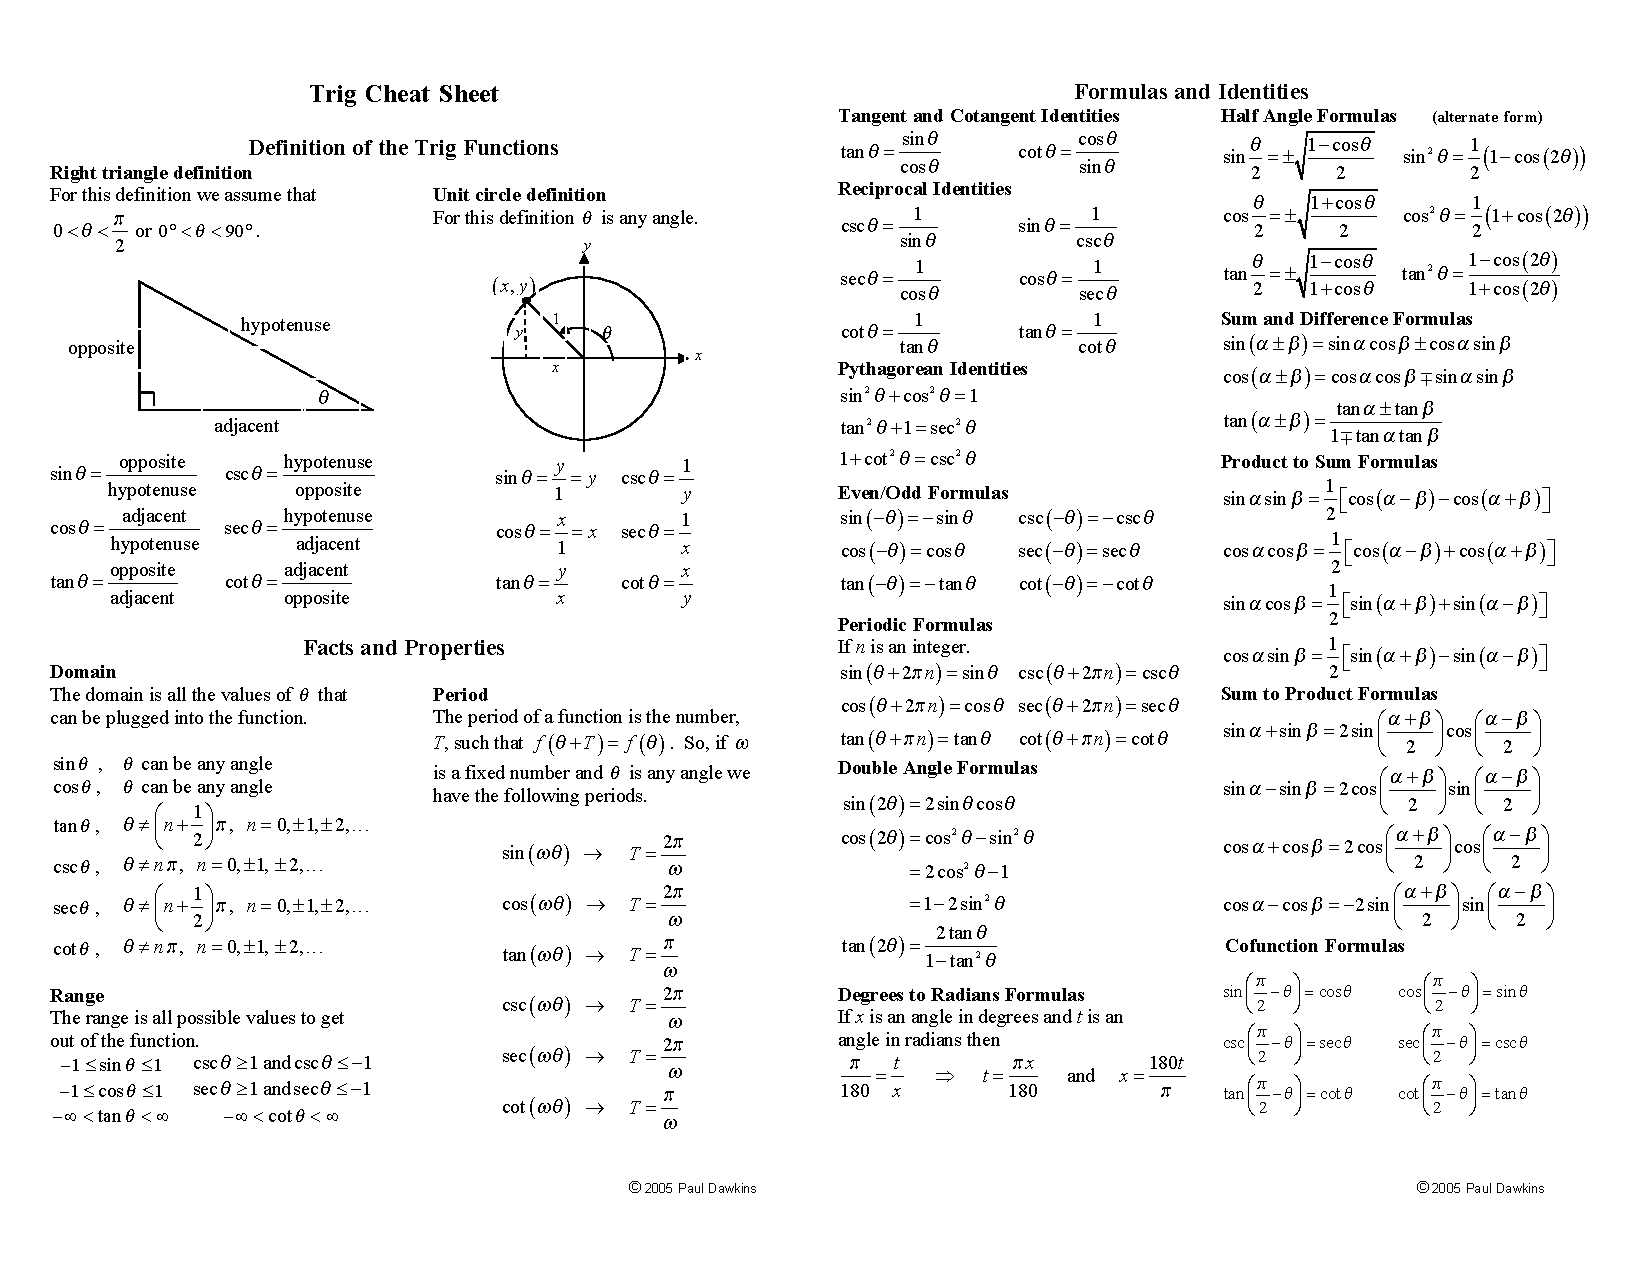
\includepdf[pages={1-},scale=1, angle=90]{Math/Trig_Cheat_Sheet_Reduced.pdf}

\end{multicols}
\end{landscape}

\end{document}
